
\section[Лексическая семантика]{Вычислительная лексическая семантика}
\subsection{ }


\begin{frame}
\frametitle{Введение}

\begin{block}{О себе}

\begin{enumerate}
\item PhD in Computational Linguistics
\begin{itemize}
    %\item co-tutelle Universit\'{e} catholique de Louvain и МГТУ им. Н.Э.Баумана;
    \item \url{http://panchenko.me}
    \item \bf{\url{alexander.panchenko@uclouvain.be}}
\end{itemize}

\item Старший исследователь в \textit{Digital Society Laboratory}.

\item Ассоциированный исследователь в \textit{Universit\'{e} catholique de
Louvain}.

\item Область научных интересов -- Natural Language Processing:

\begin{itemize}
    \item Вычислительная лексическая семантика.
    \item Классификация (коротких) текстов.
    \item АОТ для анализа социальных сетей.  
\end{itemize}


\end{enumerate}
\end{block}

\end{frame}






\begin{frame}
\frametitle{Вычислительная лексическая семантика}

\begin{figure}
\centering
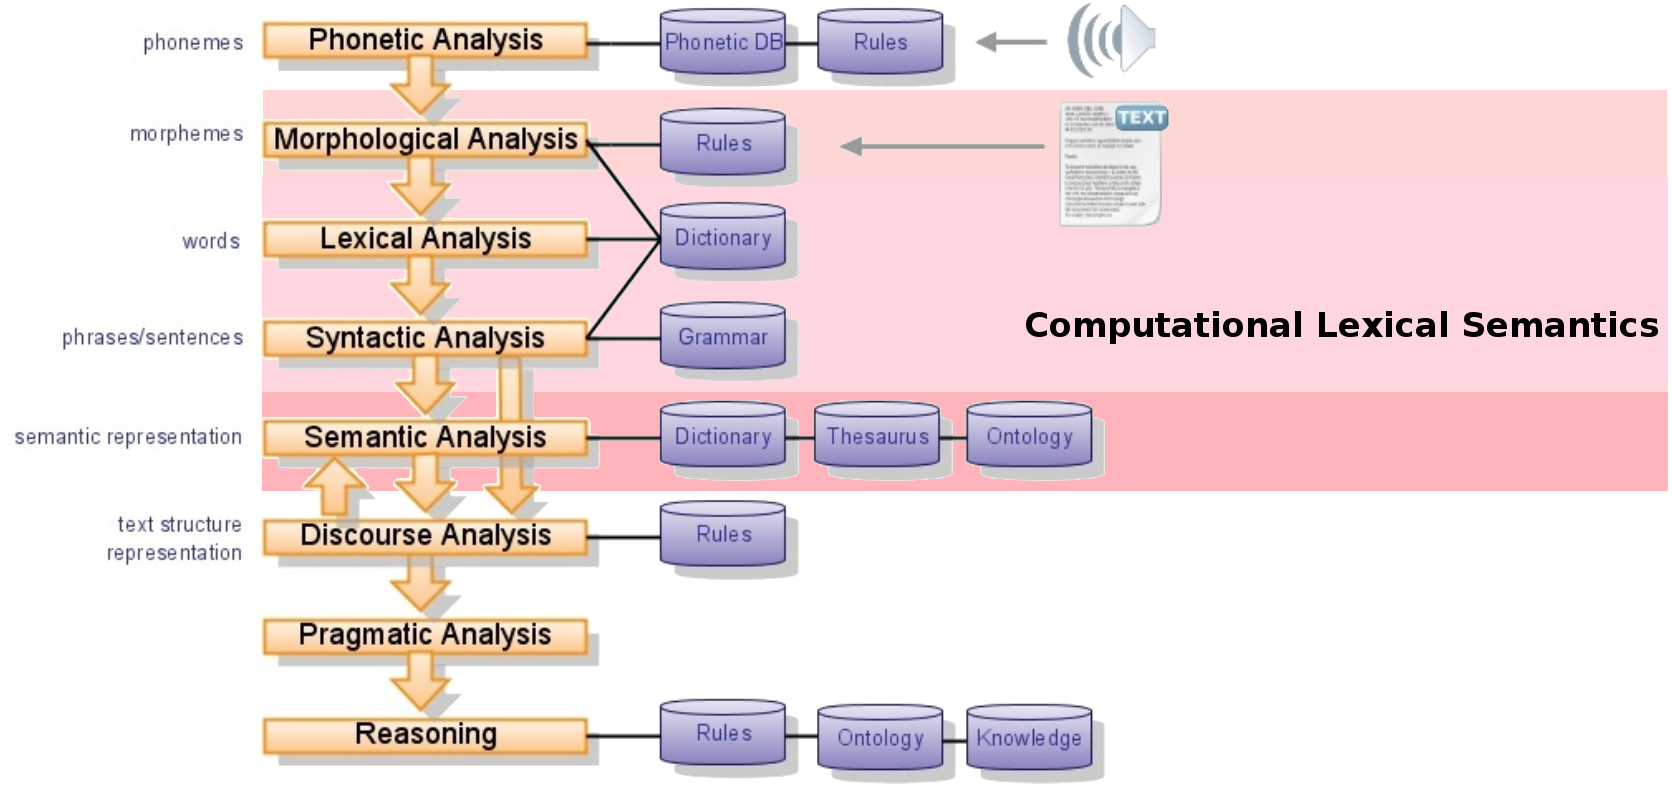
\includegraphics[width=1.05\textwidth]{./figures/levels}
\end{figure}

 \tiny{* рисунок адаптирован из курса Computational Linguistics LINGI2263 \url{http://www.uclouvain.be/en-cours-2013-LINGI2263.html}}

\end{frame}


\begin{frame}
\frametitle{Вычислительная лексическая семантика}

%\begin{block}{Вычислительная лексическая семантика изучает \ldots}
\begin{itemize}
  \item \textbf{вычислительные модели} семантики лексических единиц 
  \begin{itemize}
    \item слово
    \item именная группа
  \end{itemize}
\end{itemize}

\begin{block}{Задачи}
\begin{itemize}
  \item \textbf{word sense disambiguation}: разрешение смысла слова
  \item \textbf{named entity disambiguation}: разрешение смысла именованной сущности
  \item \textbf{semantic relation extraction}: извлечение семантических отношений 
  \item \textbf{semantic similarity}: метрики семантической близости словами 
  \item \textbf{word sense induction}: обнаружение смыслов слов 
\end{itemize}
\end{block}
\end{frame}



\begin{frame}
\frametitle{Введение в область лексической семантики}

\begin{itemize}
  \item Jurafsky D. and Martin J.H. An \textbf{Introduction to Natural Language Processing, Computational Linguistics, and Speech Recognition} (2009), chapters 19,20, 22.

\item Cruys T. \textbf{Mining for meaning: the extraction of lexico-semantic knowledge from text} (2010). PhD thesis. \url{http://dissertations.ub.rug.nl/faculties/arts/2010/t.van.de.cruys/} 

\item Panchenko A. \textbf{Similarity Measures for Semantic Relation Extraction} (2013) \url{http://cental.fltr.ucl.ac.be/team/~panchenko/thesis.pdf} 

\item \textbf{Введение в обработку текста}. ИСП РАН, ВМК МГУ, Лекция 6 и 7 \url{http://modis.ispras.ru/tpc/wp-content/uploads/2011/10/lecture6-2013.pdf} 

\end{itemize}


\end{frame}




\begin{frame}
\frametitle{Ключевые понятия}

\begin{itemize}
  \item \textbf{Лексическая единица}: слово, словосочетание, именная группа.
  \item \textbf{Лексикон}: множество слов. 
  \item \textbf{Семантическое отношение}: синонимия, гиперонимия, ассоциация, \ldots
  \item \textbf{Семантический ресурс}: лексикон + множество семантических отношений. 
  \item \textbf{Семантическая близость}: численная мера подобия смысла слов
  \item \textbf{Синсет}: множество синонимов
  \item \textbf{Смысл}: значение слова. Одному слову может соответствовать несколько смыслов.
  \item \textbf{Инвентарь смыслов:} множество соответствий между словами и смыслами. 
\end{itemize}


\end{frame}



\begin{frame}
\frametitle{Семантические отношения}
\begin{figure}
\centering
\includegraphics[width=0.65\textwidth]{./../figures/sr-29-example}
\caption{Семантический ресурс из 29 отношений.}
\end{figure}

\end{frame}






\begin{frame}
\frametitle{Семантические отношения: типы}

\begin{figure}
\centering
\includegraphics[height=0.49\textwidth]{./../figures/sr-example-2}
\includegraphics[height=0.35\textwidth]{./../figures/sr-example-spacer}
\includegraphics[height=0.43\textwidth]{./../figures/sr-example-untyped-2}
\caption{Семантический ресурс с (a) типизированными  и (b) нетипизированными  отношениями. }
\end{figure}

\end{frame}






\begin{frame}
\frametitle{Семантические отношения: типы}

\begin{figure}
\centering
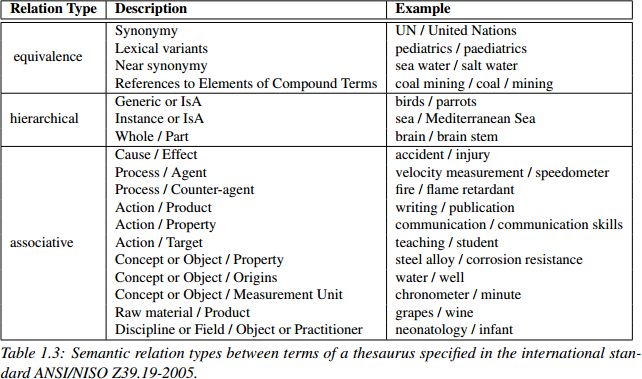
\includegraphics[height=0.49\textwidth]{./figures/sem-types}
\end{figure}

\end{frame}






\begin{frame}
\frametitle{Семантические отношения: типы}
\begin{figure}
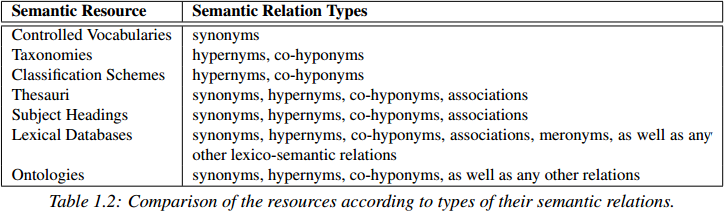
\includegraphics[width=1.0\textwidth]{figures/sem-res-table}
\end{figure}
\end{frame}


\frame{
\frametitle{Synsets}

\begin{figure}
\centering
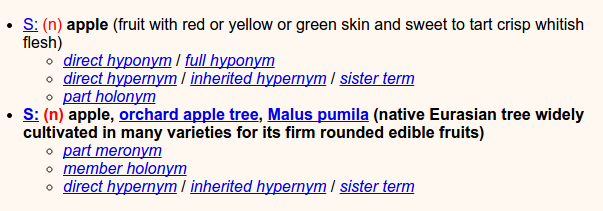
\includegraphics[width=0.9\textwidth]{figures/synset}
\caption{ WordNet synsets: \url{http://wordnetweb.princeton.edu/perl/webwn}. }
\end{figure}

}

\frame{
\frametitle{Synsets}

\begin{figure}
\centering
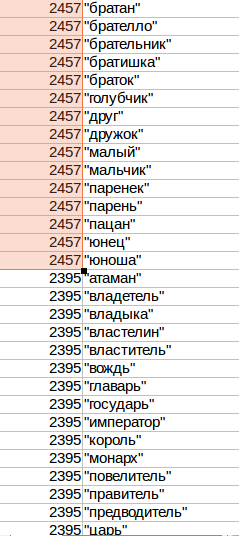
\includegraphics[width=0.26\textwidth]{figures/yarn}
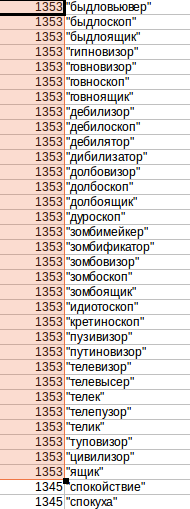
\includegraphics[width=0.22\textwidth]{figures/yarn2}
\caption{ YARN synsets: \url{http://russianword.net}. }
\end{figure}

}

\frame{
\frametitle{Synsets}

\begin{figure}
\centering
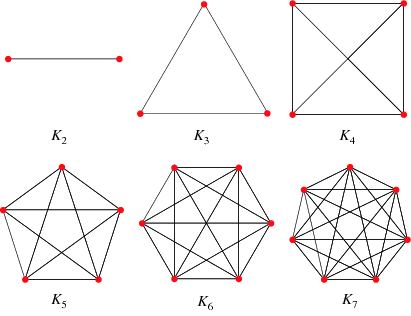
\includegraphics[width=0.7\textwidth]{figures/complete}
\caption{ Synset is a complete graph of synonyms. Source: \url{http://mathworld.wolfram.com/CompleteGraph.html}. }
\end{figure}

}

\begin{frame}
\frametitle{Семантические ресурсы: выразительность}

\begin{figure}
\centering
\includegraphics[width=0.9\textwidth]{../figures/expressivness}
\caption{ Выразительность различных моделей представления семантичеких ресурсов. }
\label{fig:expressiveness}
\end{figure}

\end{frame}





\begin{frame}
\frametitle{Семантические ресурсы: таксонония }

\begin{figure}
\centering
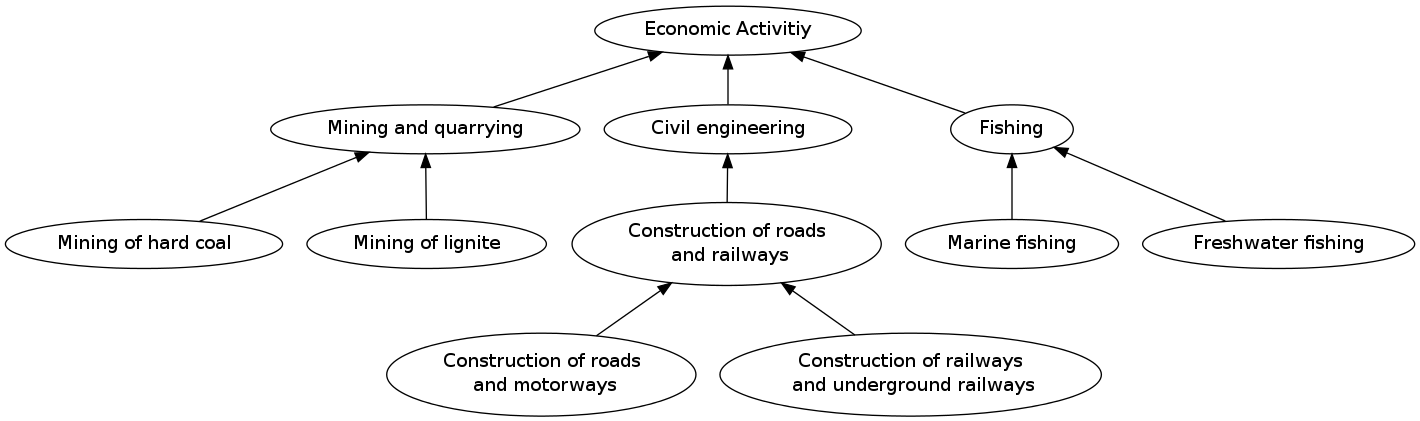
\includegraphics[width=1.0\textwidth]{../figures/taxonomy-new}
\caption{ A part of the taxonomy of economical activities NACE.}
\label{fig:taxonomy}
\end{figure}

\end{frame}





\begin{frame}
\frametitle{Семантические ресурсы: тезаурус }

\begin{figure}
\centering
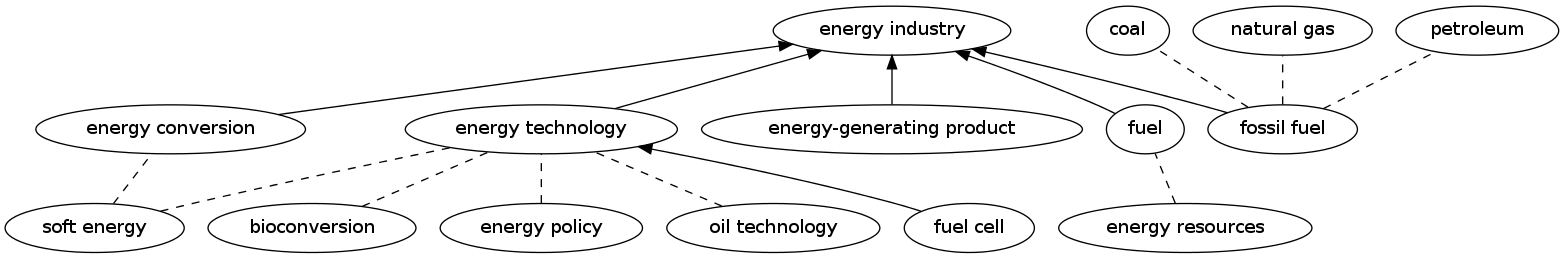
\includegraphics[width=1.0\textwidth]{../figures/thesaurus-new}
\caption{ The Eurovoc thesaurus: the term ``energy industry'' and its semantic relations. Here, hypernyms are denoted with arrows and associations are denoted with dashed lines.}
\label{fig:thesaurus}
\end{figure}
\end{frame}




\begin{frame}
\frametitle{Семантические ресурсы: лексические базы данных }

\begin{figure}
\centering
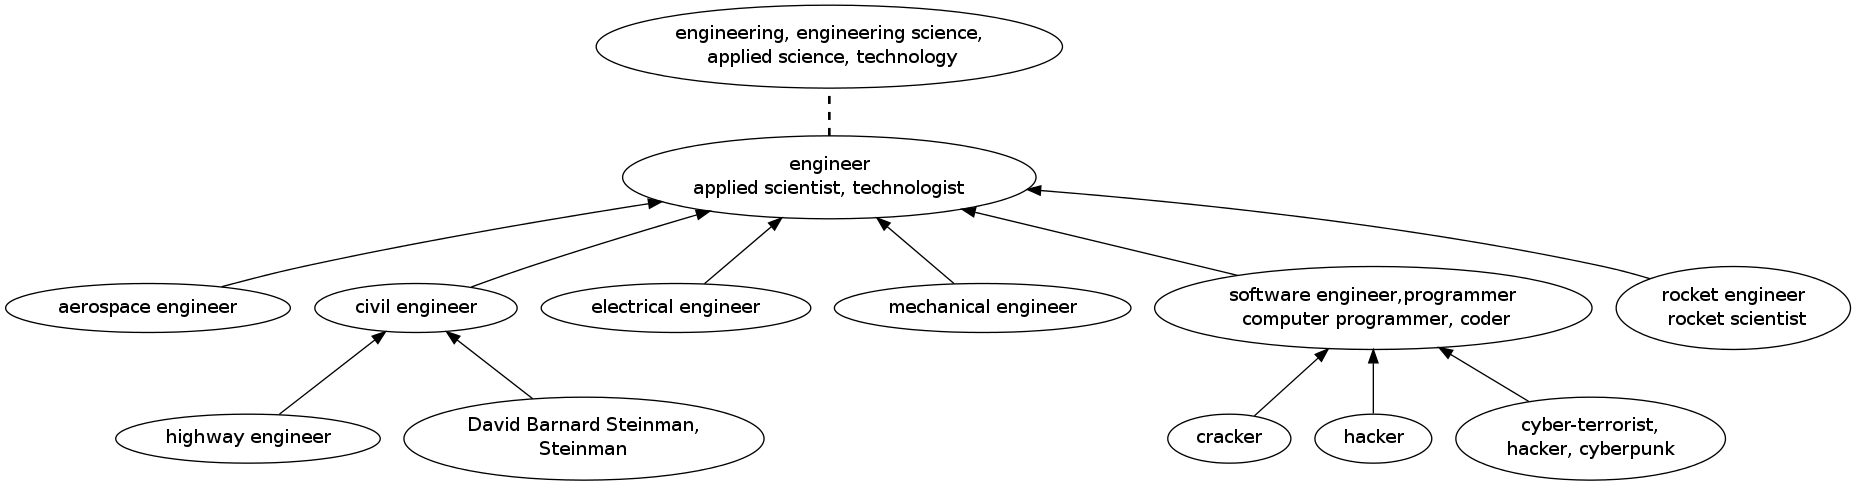
\includegraphics[width=1.0\textwidth]{../figures/wordnet-new}
\caption{ Lexical database WordNet: synset \textit{engineer} and its semantic relations. }
\label{fig:wordnet}
\end{figure}
\end{frame}


\begin{frame}
\frametitle{Семантические ресурсы: лексические базы данных }

\begin{figure}
\centering
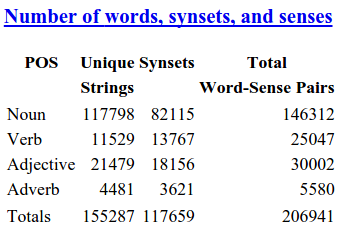
\includegraphics[width=.7\textwidth]{figures/wnstat}
\caption{ WordNet statistics. Source: \url{https://wordnet.princeton.edu/wordnet/man/wnstats.7WN.html} }
\label{fig:wordnet}
\end{figure}
\end{frame}



\begin{frame}
\frametitle{Семантические ресурсы: онтология }

\begin{figure}
    \centering
        \includegraphics[width=1.0\textwidth]{../figures/ontology-new}
    \caption{ SUMO upper ontology: a part of the class hierarchy.}
    \label{fig:sumo}
\end{figure}
\end{frame}





\begin{frame}
\frametitle{Извлечение семантических отношений из текста }

\begin{figure}
\centering
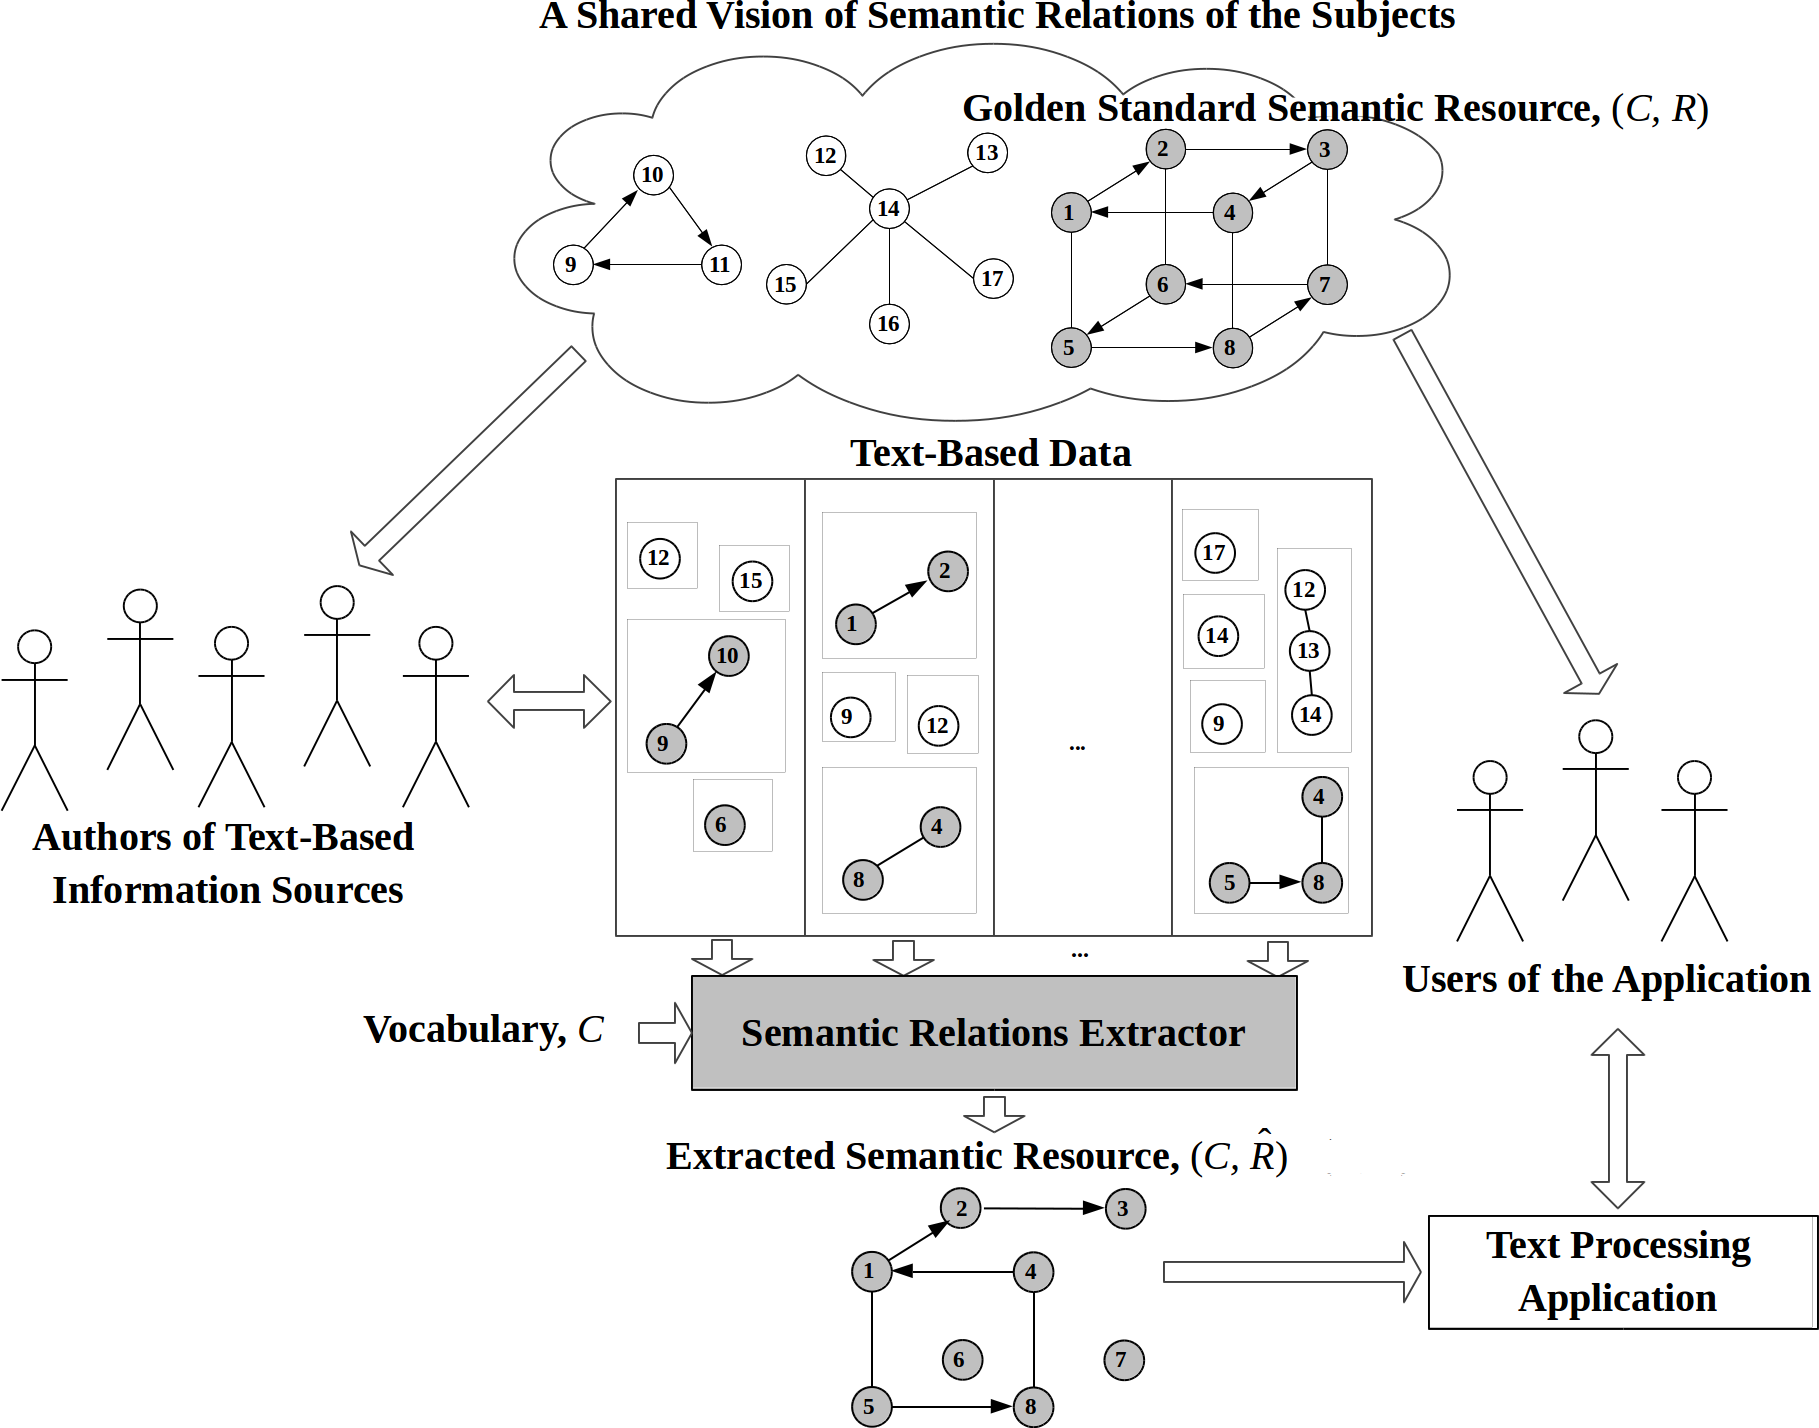
\includegraphics[width=0.8\textwidth]{../figures/extraction-3}

\label{fig:semantic-relations-extraction}
\end{figure}

\end{frame}





\begin{frame}
\frametitle{Метрики семантической близости}

\begin{block}{Мотивация исследования}

\begin{enumerate}
\item Метрики семантической близости \alert{полезны} для:
    \begin{itemize}
    \item систем обработки коротких текстов (Šaric et al., 2012; Panchenko at.,
    2012);
    \item расширешия поисковых запросов (Hsu et al., 2006);
    \item вопросно-ответных систем (Sun et al., 2005);
    \item разрешения омонимии (Patwardhan et al., 2003);
    \item \ldots 
    \end{itemize}

%\item Ручное создание семантических ресурсов непозволительно
%\alert{дорого}.
%\item  \alert{Качество} существующих систем извлечения недостаточно.
\end{enumerate}
\end{block}

\begin{itemize}
  \item Лексико-семантическое знание о языке.
  \item Вычислительная лексическая семантика.
  \item Computational Lexical Semantics. 
\end{itemize}

%\begin{block}{Focus}
%\alert{Similarity-based} semantic relation extraction.
%\end{block}

%\begin{block}{Research Question}
%How to \alert{improve} precision and coverage of such measures?
%\end{block}

\note[item]{\ldots}
\note[item]{\ldots}

\end{frame}




\frame{
\frametitle{Метрики близости }

\begin{itemize}
  \item \textbf{Similarity measure} is a numerical measure of the degree the two objects are alike  
  \item \textbf{Dissimilarity measure} is a numerical measure of the degree to which the two objects are different.
  \item Both similarity and dissimilarity scores are scalars in range $[0;1]$ or $[0;\infty]$.
  \item Two similar objects $i$ and $j$ will have a high similarity score $s_{ij}$ and a low dissimilarity score $d_{ij}$.
  \item Similarity to dissimilarity and vice versa:
 \begin{itemize}
    \item if $d_{ij} \in [0;1]$, then $s_{ij} = 1 -d_{ij}$, where $s_{ij} \in [0;1]$;
    \item if $s_{ij} \in [0;1]$, then $d_{ij} = 1 - s_{ij}$, where $d_{ij} \in [0;1]$;
    \item if $d_{ij} \in [0;\infty]$, then $s_{ij} = 1 - \frac{d_{ij} - \min_{i,j}(d_{ij})}{\max_{i,j}(d_{ij}) - \min_{i,j}(d_{ij}) }$, where $s_{ij} \in [0;1]$;
    \item if $s_{ij} \in [0;\infty]$, then $d_{ij} = 1 - \frac{s_{ij} - \min_{i,j}(s_{ij})}{\max_{i,j}(s_{ij}) - \min_{i,j}(s_{ij}) }$, where $d_{ij} \in [0;1]$.
\end{itemize}
\end{itemize} 

\textit{Definitions are adapted from (Tan, 2006).}


}

\begin{frame}
\frametitle{Метрики семантической близости}

\begin{block}{Определение}
  Метрика семантической близости численно выражает семантическую связность слов
  $c_i$ и $c_j$: $s_{ij} =
  sim(c_i,c_j)$:
    $$
  s_{ij} = \left\{ 
   \begin{array}{l l}
    \text{1} & \quad \text{если } \langle c_i, c_j \rangle \text{ -- пара }
    syn, hyper, cohypo \\
    0 & \quad \text{иначе}\\
   \end{array} \right.
 $$
 \end{block}


\begin{block}{Свойства}
\begin{itemize}    
  \item Неотрицательность: $0 \leq s_{ij} \leq 1$;
  \item Рефлективность: $s_{ij} = 1 \Leftrightarrow c_i = c_j$;
  \item Симметричность: $s_{ij} = s_{ji}$;
  \item $s_{ij} \leq s_{ik} + s_{kj}$  
  \end{itemize}
 \end{block}
     
\end{frame}



\frame{
\frametitle{Матрица подобия слов $\mathbf{S}$}


\begin{itemize}
\item $\mathbf{S}$ -- матрица подобия;
\item $s_{ij} \in \mathbf{S}$ -- мера близости слов $w_i$ и $w_j$;
\item $s_{ij} = sim(w_i, w_j), s_{ij} \in [0;1].$
\end{itemize}

\begin{figure}
\centering
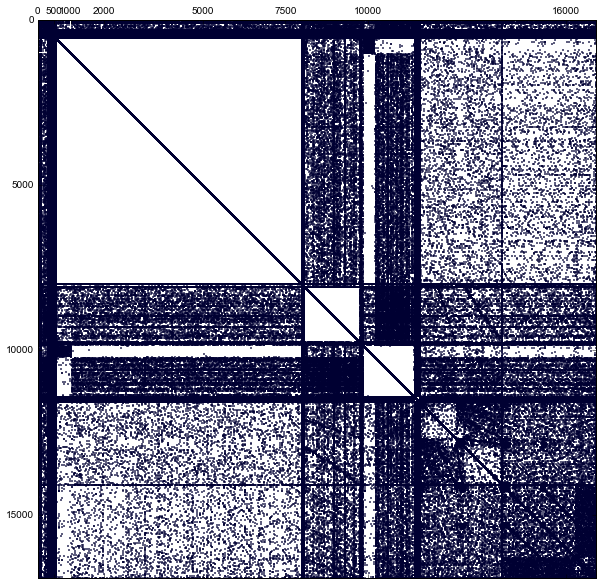
\includegraphics[width=0.5\textwidth]{./figures/simm}
\end{figure}

}



\begin{frame}
\frametitle{Метрики семантической близости: распределение}
\begin{itemize}

\item Малое количество подобных пар:
$s_{ij} \sim exp(\lambda)$.

\begin{figure}
\centering
\includegraphics[width=0.5\textwidth]{./../figures/reldist-crop}
\end{figure}

\item Распределение сем. близости слова ``doctor'':

\begin{figure}
\centering
\includegraphics[width=0.6\textwidth]{./../figures/real-extracted}
\end{figure} 

\end{itemize}
\end{frame}





\begin{frame}
\frametitle{Метрики семантической близости: распределение}
\begin{figure}
\centering
\includegraphics[width=0.9\textwidth]{./../figures/reldist}
\caption{ Number of relations (synonyms and hyponyms) per term in the dictionaries: a dictionary of synonyms, Roget's thesaurus, WordNet and a union of these three resources.  }
\label{fig:sim-distribution}
\end{figure}

\end{frame}




\begin{frame}
\frametitle{Системы измерения семантической близости}
\begin{figure}
\centering
\includegraphics[width=0.9\textwidth]{./../figures/ssr-extraction-2}
\end{figure}

\end{frame}



\frame{
\frametitle{Извлеченный и искомый семантический ресурсы}

\begin{itemize}
\item \textbf{Искомый семантический ресурс} -- это отношение: $R \subseteq C \times C$;
\item \textbf{Извлеченный семантический ресурс} -- это отношение: $\hat{R} \subseteq C \times C$.
\item \textbf{Цель} -- $\hat{R} = R$.
\item \textbf{Критерии качества} на основании $R$. 
%\item Как построить систему с высокой \textbf{точностью} и \textbf{лексическим покрытием}? 
\end{itemize}

}


\begin{frame}
\frametitle{Оценка качества метрики семантической близости}

\begin{enumerate}
\item \textbf{Корреляция с суждениями человека о сем. близости}:
\begin{itemize}
  \item Статистики: корреляция Пирсона ($\rho$) и Спирмена ($r$).
  \item Проверочные данные: MC, RG, WordSim.
\end{itemize}

\item \textbf{Ранжирование семантических отношений}:
\begin{itemize}
  \item Точность, Полнота, F-мера.
  \item Проверочные данные: BLESS, SN.
\end{itemize}


\item \textbf{Точность извлечения семантических отношений:}
\begin{itemize}
  \item Статистики: Точность@k.
  \item Проверочные данные: аннотирование и/или тезаурусы.
\end{itemize}

\item \textbf{Использование метрики в системе АОТ:}
\begin{itemize}
\item в системе классификации имен файлов (\textbf{iCOP});
\item с системе поиска семантически связанных слов (\textbf{Serelex}).
\end{itemize}
\end{enumerate}


Panchenko A., \textbf{Similarity Measures for Semantic Relation Extraction.} PhD thesis. Universit\'{e} catholique de Louvain. 197 pages, 2013, (Chapter 1). 

\end{frame}






%%%%%%%%%%%%%%%%%%%%%%%%%%%%%%%%%%%%%%%%%%%%%%%%%
%\subsection{Критерии}

%%%%%%%%%%%%%%%%%%%%%%%%%%%%%%%%%%%%%%%%%%%%%%%%%
\begin{frame}
\frametitle{Критерии, основанные на суждениях субъектов о семантической близости}

\begin{table}[h]\footnotesize
\begin{tabular}{ |c|c|c|c|c|c| }
\hline
  слово, $c_i$ & слово, $c_j$ & субъект, $\mathbf{s}$  & sim, $\mathbf{s}$  & субъект (ранг), $\mathbf{r}$ & sim (ранг), $\hat{\mathbf{r}}$  \\ \hline \hline
tiger & cat & 7.35 & 0.85 & 1 & 3 \\
book & paper & 7.46 &  0.95 & 2 & 2 \\
computer & keyboard & 7.62 &  0.81 & 3 & 1 \\
... & ... & ... & ...   & \ldots & \ldots \\
possibility & girl & 1.94 & 0.25 & 64 & 65 \\
sugar & approach & 0.88 & 0.05 & 65 & 23 \\ \hline
\end{tabular}
\end{table}


\textbf{Данные:}

\begin{itemize}
    \item WordSim353 -- 353 пар слов (Finkelstein, 2002)  
    \item MC -- 30 пар слов  (Miller & Charles, 1991)
    \item RG -- 65 пар слов (Rubenstein & Goodenough, 1965)  
\end{itemize}

\textbf{Коэффициент корреляции Пирсона:}  $\rho = \frac{cov(\mathbf{s},\hat{\mathbf{s}})}{\sigma(\mathbf{s}) \sigma(\hat{\mathbf{s}})}$

 \textbf{Коэффициент корреляции Спирмена:}: $r = \frac{cov(\mathbf{r},\hat{\mathbf{r}})}{\sigma(\mathbf{r}) \sigma(\hat{\mathbf{r}})}$
 
\end{frame}





\begin{frame}
\frametitle{Критерии, основанные на суждениях субъектов о семантической близости}

\begin{figure}
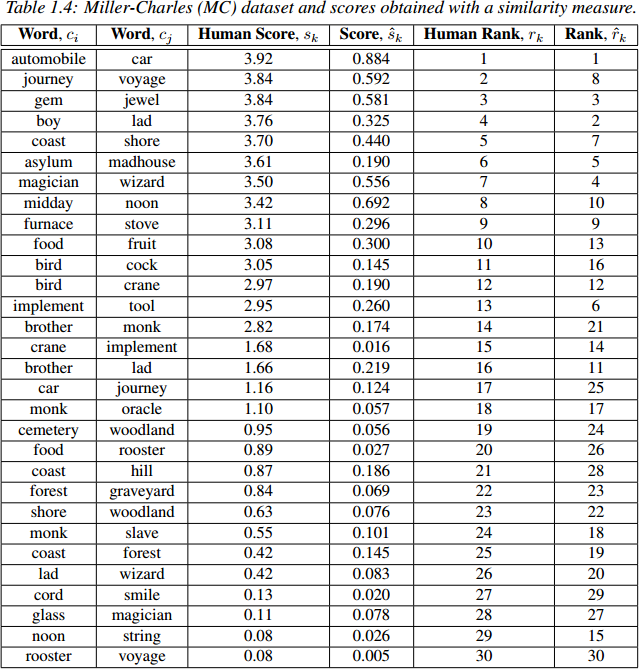
\includegraphics[height=0.6\textwidth]{./figures/rg}
\end{figure}


\end{frame}




\begin{frame}
\frametitle{Критерии, основанные на суждениях субъектов о семантической близости}

\begin{figure}
    \centering
        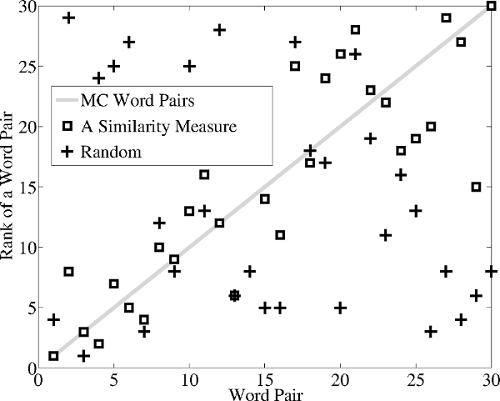
\includegraphics[width=0.55\textwidth]{../figures/mc-correlations-2}
    \caption{ Ранговая корреляция Спирмена на наборе данных Miller-Charles (MC). $\rho$ метрики равно 0.843 (p<0.001), а корреляция случайных данных -0.173 (p=0.360). }
    \label{fig:mc-correlations}
\end{figure}
\end{frame}


%%%%%%%%%%%%%%%%%%%%%%%%%%%%%%%%%%%%%%%%%%%%%%%%%
\begin{frame}
\frametitle{Критерии точности извлечения: ранжирование}

{ \scriptsize

\begin{table}[h]\footnotesize
\begin{tabular}{ |c|l|l| }
\hline
\bf слово, $c_i$ & \bf  слово, $c_j$ & \bf тип отношения, $t$  \\ \hline \hline
judge & adjudicate & syn \\
judge & arbitrate & syn \\
judge & asessor & syn \\
judge & chancellor & syn \\
judge & gendarmerie & syn \\
judge & sheriff & syn \\
... & ... & ...   \\
judge & pc & random \\ 
judge & fare & random \\
judge & lemon & random \\ \hline
\end{tabular}
\end {table}

}

\textbf{Данные:}
\begin{itemize}
  \item BLESS (Baroni and Lenci, 2011)  -- 26554 отношений (hyper, coord, mero, event, attri, random)  
  \item SN (Panchenko, 2012) -- 14682  отношений (syn, random) 
\end{itemize}

\end{frame}





%%%%%%%%%%%%%%%%%%%%%%%%%%%%%%%%%%%%%%%%%%%%%%%%%
\begin{frame}
\frametitle{Критерии точности извлечения: ранжирование}

\begin{itemize}
  
  \item Основаны на количестве \alert{правильно отранжированных} отношений.
  

\item $R$ -- все семантические отношения, не являющиеся случайными ($\langle animal, random, bishop \rangle$ и т.п.)

\item $\hat{R}(k)$ множество извлеченных отношений при количестве ближайших соседей $k$

\begin{block}{Критерии}

    
    \begin{itemize}
        \item Точность: $P(k)=$$\frac{|R \cap \hat{R}(k)|}{|\hat{R}(k)|}$,
        \item Полнота: $R(k)=$$\frac{|R \cap \hat{R}(k)|}{|R|}$,
        \item F1-мера: $F(k)= 2 \cdot \frac{P(k) \cdot R(k)}{P(k) + R(k)}$,
        %\item MAP $M(k) = \frac{1}{k}\sum^{k}_{i=1}P(i)$.
    \end{itemize}   
    \end{block}

\item Мы используем $P(10)$, $P(20)$, $P(50)$, $R(50)$.
    

\end{itemize}
    
    
\end{frame}


\begin{frame}
\frametitle{Критерии точности извлечения: ранжирование}

\begin{table*}
\centering
%\caption{A target word ``hawk" and all its relatum words from the BLESS dataset ranked by similarity score. The table on the left      contains relations retrieved with the $k$-NN threshold of 50$\%$ The whole table contains all relations of the word ($k=100\%). }
\includegraphics[width=0.6\textwidth]{../figures/bless-example}
\label{tbl:bless-example}
\end{table*}
    
\end{frame}

%%%%%%%%%%%%%%%%%%%%%%%%%%%%%%%%%%%%%%%%%%%%%%%%%
\begin{frame}
\frametitle{Пример: оценка точности извлечения отношений}

\begin{itemize}
    \item Точность $P(k=50)= \frac{1}{7} \approx 0.86 $
\end{itemize}


\begin{table}[h]\footnotesize
\begin{tabular}{ |l|l|l|l| }
\hline
\bf слово, $c_i$ & \bf  слово, $c_j$ & \bf тип отношения & \bf $s_{ij}$ \\ \hline \hline

aficionado & enthusiast & syn & 0.07197 \\
aficionado & fan & syn & 0.05195 \\
aficionado & admirer & syn & 0.01964 \\
aficionado & addict & syn & 0.01326 \\
aficionado & devotee & syn & 0.01163 \\
\alert{aficionado} & \alert{foundling} & \alert{random} & \alert{0.00777} \\
aficionado & fanatic & syn & 0.00414 \\ \hline
aficionado & adherent & syn & 0.00353 \\
aficionado & capital & random & 0.00232 \\
aficionado & statute & random & 0.00029 \\
aficionado & blot & random & 0.00025 \\
aficionado & meddler & random & 0.00005 \\
aficionado & enlargement & random & 0.00003 \\
aficionado & bawdyhouse & random &  0.00000 \\ 
\hline
\end{tabular}
\end {table}

\end{frame}

